\documentclass[22pt, a4]{article}

\usepackage[utf8]{inputenc} % allow utf-8 input
\usepackage[T1]{fontenc}    % use 8-bit T1 fonts
\usepackage{hyperref}       % hyperlinks
\usepackage{url}            % simple URL typesetting
\usepackage{booktabs}       % professional-quality tables
\usepackage{amsfonts}       % blackboard math symbols
\usepackage{nicefrac}       % compact symbols for 1/2, etc.
\usepackage{microtype}      % microtypography
\usepackage{graphicx}
\usepackage{xepersian}
\settextfont{XB Roya}

\renewcommand{\baselinestretch}{1.25}

\title{\lr{UML Diagrams}}

\author{%
  علیرضا سلطانی نشان\\
  دانشکده شمسی پور\\
  مهندسی نرم افزار\\
  \texttt{asn80.asn@hotmail.com}
}
\begin{document}
\maketitle
\tableofcontents

\newpage

\section{کاربرد زبان مدل سازی یکپارچه}
به طور کلی، دیاگرام
UML
یک زبان مدل سازی تحت عنوان چند منظوره در رشته مهندسی نرم افزار است.
به هر حال از آن برای جریانات کاری
\footnote{Workflows}
و فرایند های کسب و کاری 
\footnote{Business Processes}
استفاده  می کنند. برای مثال از دیاگرام اکتیویتی، که نوعی از نمودار های 
UML
است، میتواند جایگزینی بسیار مناسب برای نمودار های فلوچارت باشد .
مهم این است که هر دوی آنها در حال صحبت از یک استاندارد هستند، که
نمودار اکتیویتی میتواند محدوده بیشتری از ویژگی ها برای خوانایی و فهم بیشتری را به همراه داشته باشد.\\


UML
استفاده های زیادی را در توسعه نرم افزار و مستندات فرایند های تجاری و کسب و کاری را پیدا کرده است:

\subsection{Sketch}
نمودار UML
در این مورد برای برقراری ارتباط جنبه ها و ویژگی های مختلف یک سیستم استفاده میشود.
با این حال این مورد یک نمای سطح بالا، از سیستم است و به احتمال زیاد شامل تمام جزئیات لازم برای اجرای پروژه تا پایان کار نیست.


\subsubsection{\lr{Forward Design}}
در طراحی پیشرونده (رو به جلو)
طراحی اسکچ قبل از انجام هرگونه کودینگ یک برنامه کاربردی، صورت میگیرد. 
انجام این کار باعث میشود که شما یک ویو یا چشم اندازی بهتر و روشن تری از سیستم یا ورکفلویی که شما قصد ایجاد آنرا دارید، داشته باشید.
در طی این فرایند طراحی رو به جلو بیشتر مشکلات، مسائل، چالش ها آشکار میشوند.
بنابرین باعث میشود که از ماهیت و کلیت پروژه سر در بیاوریم و بدون هیچ گونه مشکل و استرس نداستن از چه کار کردن.

\subsubsection{\lr{Backward Design}}
طراحی رو به عقب بعد از نوشتن کد های برنامه مورد استفاده قرار میگیرد.
پس شروع میکنیم به کشیدن نمودار های یو ام ال،  به عناون فرمی ا زمستندات برای برای فعالیت های مختلف، نقش ها و اکتر ها و گردش کار های مختلف.


\subsection{طراحی اولیه}
طراحی اولیه
\footnote{Blueprint}
  .به عنوان یک طراحی کامل که صرفاً به پیاده سازی واقعی سیستم یا نرم افزار نیاز دارد ، عمل می کند.
معمولا در این روش از ابزار های مهندسی نرم افزار به کمک کامپیوتر 
\footnote{\lr{Computer Aided Software Engineering Tools}}
استفاده میشود.
اشکالی که در این حالت یعنی استفاده از ابزار ها وجود دارد، آن است که اگر آموزش
تخصصي قبلي در رابطه با اين نرم افزار ها وجود نداشته باشد، برای توسعه دهنده مدیریت
زمان مسئله ساز خواهد شد.

\subsection{زبان شبه برنامه نویسی \lr{Pseudo Programming Language}}
UML
یک زبان برنامه نویسی مستقل مثل پایتون و جاوا، سی پلاس پلاس نیست!
با این حال ، با استفاده از ابزار های مناسب، میتوان به صورت شبه کد به عنوان یک زبان شبه برنامه نویسی باید به آن نگاه کرد
برای دستیابی به این هدف، کل سیستم باید در نمودار های مختلف یو ام ال کشیده شوند، و با 
استفاده از نرم افزار های مناسب نمودار ها به طور مستقیم به کد ترجمه شوند.
حقیقتی که در این زمینه وجود دارد این است که زمان بیشتری باید برای نوشتن نمودار صرف شود تا نوشتن کد واقعی.

% \section{طراحی}

% \subsection{\lr{Software Development Methods}}

% \subsection{Modeling}

\newpage

\section{دیاگرام رفتاری}
نمودار های رفتاری شامل تعامل ها، فعالیت ها و ماشین های حالت است. نمودار های رفتاری
برای نمایش نحوه رفتاری سیستم استفاده میشود.
\subsection{\lr{Activity Diagram}}
فعالیت چیست؟\\
فعالیت عملی است که توسط انسان یا ماشین انجام میشود که در دیدگاه پیاده سازی متد است.
از این نمودار زمانی استفاده میشود که میخواهیم جریان کنترل از یک فعالیت به فعالیت دیگر را نشان دهیم و معمولا در جریان کار هایی است که به صورت موازی در حال انجام عملیاتی هستند که ممکن است در اثر بروز شرایطی رد یا پذیرفته شوند.
\\
{\par\center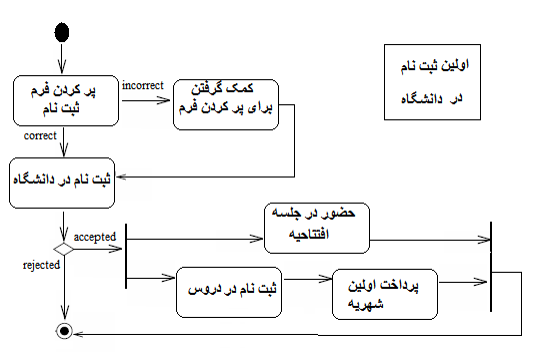
\includegraphics[width=250pt]{img/activity_diagram.png}\par}

\newpage

\newpage
\subsection{\lr{State Machine Diagram}}

از این نمودار برای نمایش حالت های مختلفی که یک کامپوننت در طی فعالیت ها و فرایند ها میتواند از خود نشان دهد استفاده میشود.
مثلا قسمتی از یک نرم افزار اموزشی که در یک روز و زمان مشخصی اجازه امتحان داد را به دانشجویان میدهد و بعد از مدتی این اجازه را از بین میبرد و از حالت باز بودن گیت ورودی به امتحان به بسته بودن تغییر میکند و  درطی مراحلی دوباره
از خود تغییر شکل نشان میدهد و آنهم نشان دادن نمره امتحان دانشجوست.\\

یا در مثالی واضح تر، وضعیت یک فرد برای گرفتن پول از دستگاه ATM.
مثلا وضعیت هایی که این فرد میتواند داشته باشد، مانند در دست داشتن کارت،
وارد کردن کارت، 
وارد کردن گزرواژه،
انتخاب حساب و انتخاب مبلغ مورد نظر باشد.

{\par\center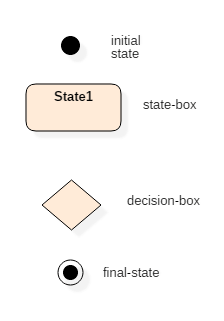
\includegraphics[width=150pt]{img/08-041519_1219_UMLNotation10.png}\par}

\newpage
\subsection{\lr{Use Case Diagram}}
این نمودار نشان دهنده روابط بین بازیگران مثلا کاربران با هم دیگر است.
یک نمودار
\lr{Use Case}
Acter
ها (کاربر ها) مختلف سیستم را در ارتباط با موارد کاربردی متفاوت نمایش میدهد.

{\par\center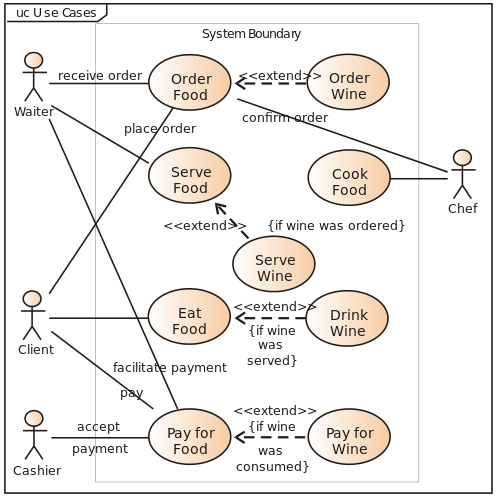
\includegraphics[width=250pt]{img/496px-Use_case_restaurant_model.svg.png}\par}

\newpage
\subsection{\lr{Timing Diagram}}
نمودار های زمانی رفتار های مختلف اشیا را در یک دوره زمانی مشخص نشان میدهد.





\end{document}

